\documentclass{beamer}
\usetheme{Boadilla}
\usepackage[utf8]{inputenc}

\title{GIS Community Outreach}
\institute{University of Auckland}
\date{Thursday 17-06-2021}

\begin{document}

\begin{frame}
\titlepage
\end{frame}

\begin{frame}{Introduction}
Kia ora!
\vspace{1cm}

\begin{minipage}{.5\textwidth}
  \centering
  Sophie Kolston\\
  \tiny she/her
  \noindent
  \begin{figure}
    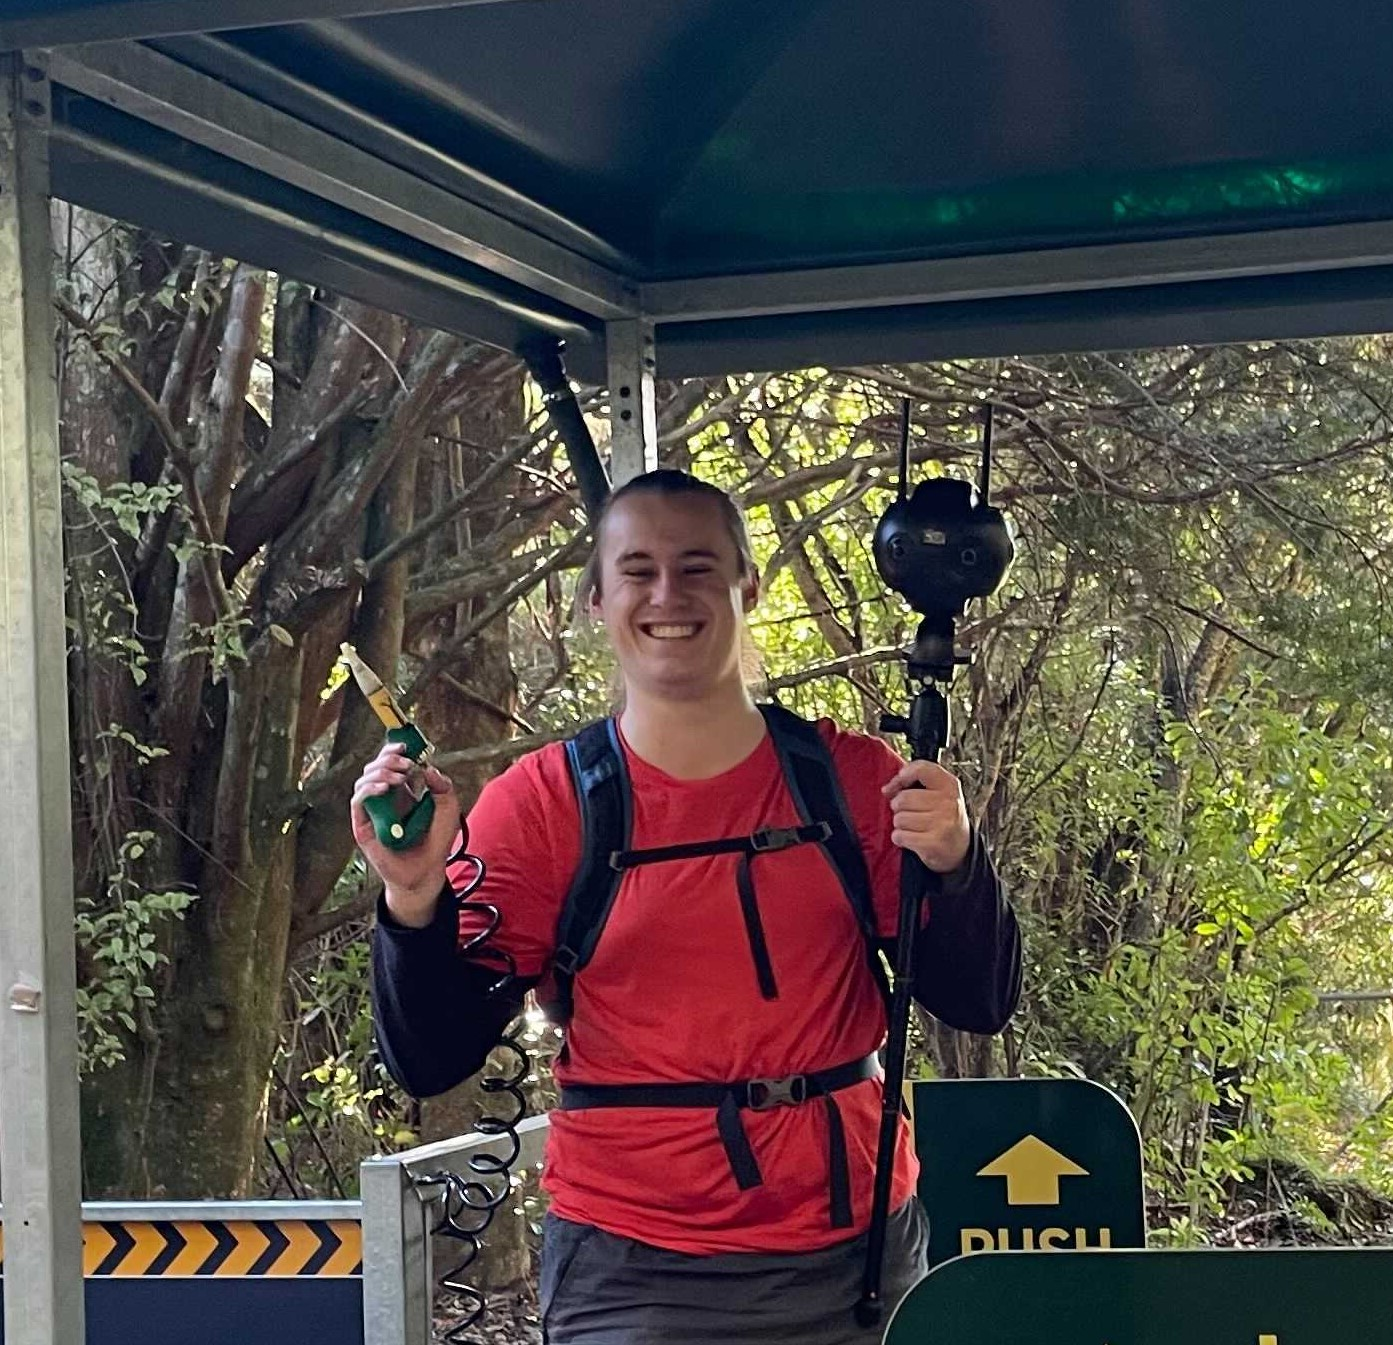
\includegraphics[width=100px]{images/sophie_cropped.jpg}
  \end{figure}
  \tiny BSc student in GIScience. Research interests in spatial programming and virtual reality.
\end{minipage}% test
\begin{minipage}{.5\textwidth}
  \centering
  Wila Wu\\
  \tiny she/her
  \noindent
  \begin{figure}
    
\includegraphics[width=96px]{images/wila.PNG}
  \end{figure}
  \tiny BSc(hons) student in Geography, focussing on human mobility in Auckland during the Covid-19 pandemic.
\end{minipage}

\end{frame}

\begin{frame}{The Plan for Today}
    \textbf{Schedule}\\
    0900-1030 Our Introduction, Lesson 1: Introduction to GIS\\
    1030-1100 Break\\
    1100-1300 Lesson 2: Vector Data Analysis\\
    1300-1400 Lunch\\
    1400-1530 Lesson 3: Raster Data Analysis\\
    1530-1600 Break\\
    1600-1700 Lesson 3 Continued, Wrap-up
\end{frame}

\begin{frame}{Objectives}
    Understanding of GISystems and Science in High School! \\
    \vspace{1cm}
    Lots of flexibility in NCEA to implement everything we will be teaching today into your geography curriculum:
    \vspace{0.5cm}
    
    \centering
    \scriptsize
    \begin{tabular}{|p{1cm}|p{2cm}|p{1cm}|p{5cm}|}
        \hline
        Level & ID & Credits & Description  \\
        \hline 
        1 & AS91014 & 3 &  Apply spatial analysis, with direction, to solve a geographic problem \\
        \hline
        2 & AS91247 & 3 & Apply spatial analysis, with guidance, to solve a geographic problem \\
        \hline
        3 & AS91433 & 3 & Apply spatial analysis, with consultation, to solve a geographic problem \\
        \hline
    \end{tabular}
\end{frame}

\begin{frame}{Objectives: Example}
\begin{minipage}{.5\textwidth}
  \centering
  \begin{figure}
    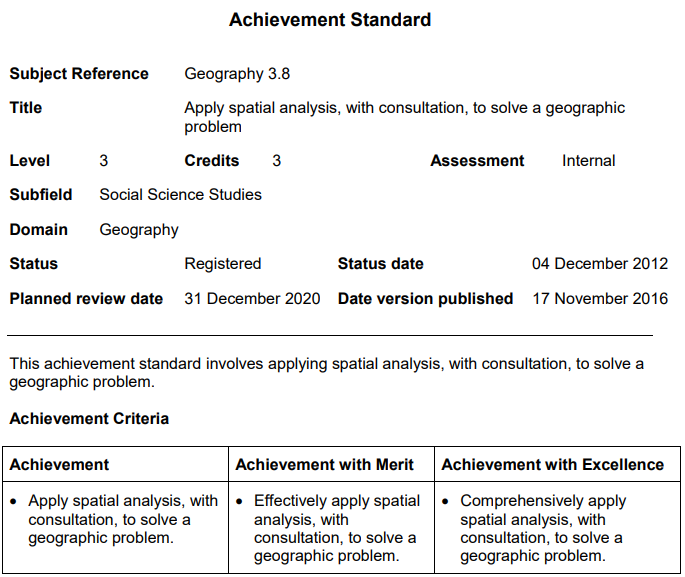
\includegraphics[width=150px]{images/standard_example.PNG}\\
    
    ...
    
    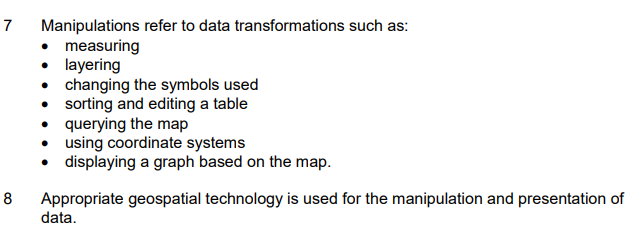
\includegraphics[width=150px]{images/standard_example_2.PNG}\\
  \end{figure}
\end{minipage}% test
\begin{minipage}{.5\textwidth}
  We will be covering everything that is required for all year levels of assessment (and more!)\\
  
  $\leftarrow$ Introduction lesson achieves this \\
  
  Ambiguous definitions, can involve physical and/or human geography
\end{minipage}
\end{frame}

\begin{frame}{Let's Get Started!}
    Any questions? 
\end{frame}

\end{document}
